
%% bare_conf.tex
%% V1.3
%% 2007/01/11
%% by Michael Shell
%% See:
%% http://www.michaelshell.org/
%% for current contact information.
%%
%% This is a skeleton file demonstrating the use of IEEEtran.cls
%% (requires IEEEtran.cls version 1.7 or later) with an IEEE conference paper.
%%
%% Support sites:
%% http://www.michaelshell.org/tex/ieeetran/
%% http://www.ctan.org/tex-archive/macros/latex/contrib/IEEEtran/
%% and
%% http://www.ieee.org/

%%*************************************************************************
%% Legal Notice:
%% This code is offered as-is without any warranty either expressed or
%% implied; without even the implied warranty of MERCHANTABILITY or
%% FITNESS FOR A PARTICULAR PURPOSE! 
%% User assumes all risk.
%% In no event shall IEEE or any contributor to this code be liable for
%% any damages or losses, including, but not limited to, incidental,
%% consequential, or any other damages, resulting from the use or misuse
%% of any information contained here.
%%
%% All comments are the opinions of their respective authors and are not
%% necessarily endorsed by the IEEE.
%%
%% This work is distributed under the LaTeX Project Public License (LPPL)
%% ( http://www.latex-project.org/ ) version 1.3, and may be freely used,
%% distributed and modified. A copy of the LPPL, version 1.3, is included
%% in the base LaTeX documentation of all distributions of LaTeX released
%% 2003/12/01 or later.
%% Retain all contribution notices and credits.
%% ** Modified files should be clearly indicated as such, including  **
%% ** renaming them and changing author support contact information. **
%%
%% File list of work: IEEEtran.cls, IEEEtran_HOWTO.pdf, bare_adv.tex,
%%                    bare_conf.tex, bare_jrnl.tex, bare_jrnl_compsoc.tex
%%*************************************************************************

% *** Authors should verify (and, if needed, correct) their LaTeX system  ***
% *** with the testflow diagnostic prior to trusting their LaTeX platform ***
% *** with production work. IEEE's font choices can trigger bugs that do  ***
% *** not appear when using other class files.                            ***
% The testflow support page is at:
% http://www.michaelshell.org/tex/testflow/



% Note that the a4paper option is mainly intended so that authors in
% countries using A4 can easily print to A4 and see how their papers will
% look in print - the typesetting of the document will not typically be
% affected with changes in paper size (but the bottom and side margins will).
% Use the testflow package mentioned above to verify correct handling of
% both paper sizes by the user's LaTeX system.
%
% Also note that the "draftcls" or "draftclsnofoot", not "draft", option
% should be used if it is desired that the figures are to be displayed in
% draft mode.
%
\documentclass[conference]{IEEEtran}
% Add the compsoc option for Computer Society conferences.
%
% If IEEEtran.cls has not been installed into the LaTeX system files,
% manually specify the path to it like:
% \documentclass[conference]{../sty/IEEEtran}





% Some very useful LaTeX packages include:
% (uncomment the ones you want to load)


% *** MISC UTILITY PACKAGES ***
%
%\usepackage{ifpdf}
% Heiko Oberdiek's ifpdf.sty is very useful if you need conditional
% compilation based on whether the output is pdf or dvi.
% usage:
% \ifpdf
%   % pdf code
% \else
%   % dvi code
% \fi
% The latest version of ifpdf.sty can be obtained from:
% http://www.ctan.org/tex-archive/macros/latex/contrib/oberdiek/
% Also, note that IEEEtran.cls V1.7 and later provides a builtin
% \ifCLASSINFOpdf conditional that works the same way.
% When switching from latex to pdflatex and vice-versa, the compiler may
% have to be run twice to clear warning/error messages.






% *** CITATION PACKAGES ***
%
%\usepackage{cite}
% cite.sty was written by Donald Arseneau
% V1.6 and later of IEEEtran pre-defines the format of the cite.sty package
% \cite{} output to follow that of IEEE. Loading the cite package will
% result in citation numbers being automatically sorted and properly
% "compressed/ranged". e.g., [1], [9], [2], [7], [5], [6] without using
% cite.sty will become [1], [2], [5]--[7], [9] using cite.sty. cite.sty's
% \cite will automatically add leading space, if needed. Use cite.sty's
% noadjust option (cite.sty V3.8 and later) if you want to turn this off.
% cite.sty is already installed on most LaTeX systems. Be sure and use
% version 4.0 (2003-05-27) and later if using hyperref.sty. cite.sty does
% not currently provide for hyperlinked citations.
% The latest version can be obtained at:
% http://www.ctan.org/tex-archive/macros/latex/contrib/cite/
% The documentation is contained in the cite.sty file itself.






% *** GRAPHICS RELATED PACKAGES ***
%
\ifCLASSINFOpdf
   \usepackage[pdftex]{graphicx}
  % declare the path(s) where your graphic files are
  % \graphicspath{{../pdf/}{../jpeg/}}
  % and their extensions so you won't have to specify these with
  % every instance of \includegraphics
  % \DeclareGraphicsExtensions{.pdf,.jpeg,.png}
\else
  % or other class option (dvipsone, dvipdf, if not using dvips). graphicx
  % will default to the driver specified in the system graphics.cfg if no
  % driver is specified.
   \usepackage[dvips]{graphicx}
  % declare the path(s) where your graphic files are
  % \graphicspath{{../eps/}}
  % and their extensions so you won't have to specify these with
  % every instance of \includegraphics
  % \DeclareGraphicsExtensions{.eps}
\fi
% graphicx was written by David Carlisle and Sebastian Rahtz. It is
% required if you want graphics, photos, etc. graphicx.sty is already
% installed on most LaTeX systems. The latest version and documentation can
% be obtained at: 
% http://www.ctan.org/tex-archive/macros/latex/required/graphics/
% Another good source of documentation is "Using Imported Graphics in
% LaTeX2e" by Keith Reckdahl which can be found as epslatex.ps or
% epslatex.pdf at: http://www.ctan.org/tex-archive/info/
%
% latex, and pdflatex in dvi mode, support graphics in encapsulated
% postscript (.eps) format. pdflatex in pdf mode supports graphics
% in .pdf, .jpeg, .png and .mps (metapost) formats. Users should ensure
% that all non-photo figures use a vector format (.eps, .pdf, .mps) and
% not a bitmapped formats (.jpeg, .png). IEEE frowns on bitmapped formats
% which can result in "jaggedy"/blurry rendering of lines and letters as
% well as large increases in file sizes.
%
% You can find documentation about the pdfTeX application at:
% http://www.tug.org/applications/pdftex





% *** MATH PACKAGES ***
%
%\usepackage[cmex10]{amsmath}
% A popular package from the American Mathematical Society that provides
% many useful and powerful commands for dealing with mathematics. If using
% it, be sure to load this package with the cmex10 option to ensure that
% only type 1 fonts will utilized at all point sizes. Without this option,
% it is possible that some math symbols, particularly those within
% footnotes, will be rendered in bitmap form which will result in a
% document that can not be IEEE Xplore compliant!
%
% Also, note that the amsmath package sets \interdisplaylinepenalty to 10000
% thus preventing page breaks from occurring within multiline equations. Use:
%\interdisplaylinepenalty=2500
% after loading amsmath to restore such page breaks as IEEEtran.cls normally
% does. amsmath.sty is already installed on most LaTeX systems. The latest
% version and documentation can be obtained at:
% http://www.ctan.org/tex-archive/macros/latex/required/amslatex/math/





% *** SPECIALIZED LIST PACKAGES ***
%
%\usepackage{algorithmic}
% algorithmic.sty was written by Peter Williams and Rogerio Brito.
% This package provides an algorithmic environment fo describing algorithms.
% You can use the algorithmic environment in-text or within a figure
% environment to provide for a floating algorithm. Do NOT use the algorithm
% floating environment provided by algorithm.sty (by the same authors) or
% algorithm2e.sty (by Christophe Fiorio) as IEEE does not use dedicated
% algorithm float types and packages that provide these will not provide
% correct IEEE style captions. The latest version and documentation of
% algorithmic.sty can be obtained at:
% http://www.ctan.org/tex-archive/macros/latex/contrib/algorithms/
% There is also a support site at:
% http://algorithms.berlios.de/index.html
% Also of interest may be the (relatively newer and more customizable)
% algorithmicx.sty package by Szasz Janos:
% http://www.ctan.org/tex-archive/macros/latex/contrib/algorithmicx/




% *** ALIGNMENT PACKAGES ***
%
%\usepackage{array}
% Frank Mittelbach's and David Carlisle's array.sty patches and improves
% the standard LaTeX2e array and tabular environments to provide better
% appearance and additional user controls. As the default LaTeX2e table
% generation code is lacking to the point of almost being broken with
% respect to the quality of the end results, all users are strongly
% advised to use an enhanced (at the very least that provided by array.sty)
% set of table tools. array.sty is already installed on most systems. The
% latest version and documentation can be obtained at:
% http://www.ctan.org/tex-archive/macros/latex/required/tools/


%\usepackage{mdwmath}
%\usepackage{mdwtab}
% Also highly recommended is Mark Wooding's extremely powerful MDW tools,
% especially mdwmath.sty and mdwtab.sty which are used to format equations
% and tables, respectively. The MDWtools set is already installed on most
% LaTeX systems. The lastest version and documentation is available at:
% http://www.ctan.org/tex-archive/macros/latex/contrib/mdwtools/


% IEEEtran contains the IEEEeqnarray family of commands that can be used to
% generate multiline equations as well as matrices, tables, etc., of high
% quality.


%\usepackage{eqparbox}
% Also of notable interest is Scott Pakin's eqparbox package for creating
% (automatically sized) equal width boxes - aka "natural width parboxes".
% Available at:
% http://www.ctan.org/tex-archive/macros/latex/contrib/eqparbox/





% *** SUBFIGURE PACKAGES ***
%\usepackage[tight,footnotesize]{subfigure}
% subfigure.sty was written by Steven Douglas Cochran. This package makes it
% easy to put subfigures in your figures. e.g., "Figure 1a and 1b". For IEEE
% work, it is a good idea to load it with the tight package option to reduce
% the amount of white space around the subfigures. subfigure.sty is already
% installed on most LaTeX systems. The latest version and documentation can
% be obtained at:
% http://www.ctan.org/tex-archive/obsolete/macros/latex/contrib/subfigure/
% subfigure.sty has been superceeded by subfig.sty.



%\usepackage[caption=false]{caption}
%\usepackage[font=footnotesize]{subfig}
% subfig.sty, also written by Steven Douglas Cochran, is the modern
% replacement for subfigure.sty. However, subfig.sty requires and
% automatically loads Axel Sommerfeldt's caption.sty which will override
% IEEEtran.cls handling of captions and this will result in nonIEEE style
% figure/table captions. To prevent this problem, be sure and preload
% caption.sty with its "caption=false" package option. This is will preserve
% IEEEtran.cls handing of captions. Version 1.3 (2005/06/28) and later 
% (recommended due to many improvements over 1.2) of subfig.sty supports
% the caption=false option directly:
%\usepackage[caption=false,font=footnotesize]{subfig}
%
% The latest version and documentation can be obtained at:
% http://www.ctan.org/tex-archive/macros/latex/contrib/subfig/
% The latest version and documentation of caption.sty can be obtained at:
% http://www.ctan.org/tex-archive/macros/latex/contrib/caption/




% *** FLOAT PACKAGES ***
%
%\usepackage{fixltx2e}
% fixltx2e, the successor to the earlier fix2col.sty, was written by
% Frank Mittelbach and David Carlisle. This package corrects a few problems
% in the LaTeX2e kernel, the most notable of which is that in current
% LaTeX2e releases, the ordering of single and double column floats is not
% guaranteed to be preserved. Thus, an unpatched LaTeX2e can allow a
% single column figure to be placed prior to an earlier double column
% figure. The latest version and documentation can be found at:
% http://www.ctan.org/tex-archive/macros/latex/base/



%\usepackage{stfloats}
% stfloats.sty was written by Sigitas Tolusis. This package gives LaTeX2e
% the ability to do double column floats at the bottom of the page as well
% as the top. (e.g., "\begin{figure*}[!b]" is not normally possible in
% LaTeX2e). It also provides a command:
%\fnbelowfloat
% to enable the placement of footnotes below bottom floats (the standard
% LaTeX2e kernel puts them above bottom floats). This is an invasive package
% which rewrites many portions of the LaTeX2e float routines. It may not work
% with other packages that modify the LaTeX2e float routines. The latest
% version and documentation can be obtained at:
% http://www.ctan.org/tex-archive/macros/latex/contrib/sttools/
% Documentation is contained in the stfloats.sty comments as well as in the
% presfull.pdf file. Do not use the stfloats baselinefloat ability as IEEE
% does not allow \baselineskip to stretch. Authors submitting work to the
% IEEE should note that IEEE rarely uses double column equations and
% that authors should try to avoid such use. Do not be tempted to use the
% cuted.sty or midfloat.sty packages (also by Sigitas Tolusis) as IEEE does
% not format its papers in such ways.





% *** PDF, URL AND HYPERLINK PACKAGES ***
%
%\usepackage{url}
% url.sty was written by Donald Arseneau. It provides better support for
% handling and breaking URLs. url.sty is already installed on most LaTeX
% systems. The latest version can be obtained at:
% http://www.ctan.org/tex-archive/macros/latex/contrib/misc/
% Read the url.sty source comments for usage information. Basically,
% \url{my_url_here}.





% *** Do not adjust lengths that control margins, column widths, etc. ***
% *** Do not use packages that alter fonts (such as pslatex).         ***
% There should be no need to do such things with IEEEtran.cls V1.6 and later.
% (Unless specifically asked to do so by the journal or conference you plan
% to submit to, of course. )


% correct bad hyphenation here
\hyphenation{op-tical net-works semi-conduc-tor}

\newcommand{\Nemico}{{\sc NeMiCo}} 
\newcommand{\NemicoDef}{{\sc Ne}twork {\sc Mi}ning in the {\sc C}l{\sc o}ud} 

\newcommand{\comment}[1]{} 

\begin{document}
%
% paper title
% can use linebreaks \\ within to get better formatting as desired
\title{{\Nemico : Mining network data through cloud-based data mining techniques}}


% author names and affiliations
% use a multiple column layout for up to three different
% affiliations


% conference papers do not typically use \thanks and this command
% is locked out in conference mode. If really needed, such as for
% the acknowledgment of grants, issue a \IEEEoverridecommandlockouts
\author{\IEEEauthorblockN{Elena Baralis, Luca Cagliero, Tania Cerquitelli, Silvia Chiusano, Paolo Garza, Luigi Grimaudo, Fabio Pulvirenti}
\IEEEauthorblockA{Dipartimento di Automatica e Informatica\\
Politecnico di Torino - Torino, Italy\\
Email: \{name.surname\}@polito.it}
\thanks{The research leading to these results has received funding from the European Union 
under the FP7 Grant Agreement n. 619633 (Integrated Project ''ONTIC'')
}}

\IEEEoverridecommandlockouts

% after \documentclass

% for over three affiliations, or if they all won't fit within the width
% of the page, use this alternative format:
% 
%\author{\IEEEauthorblockN{Michael Shell\IEEEauthorrefmark{1},
%Homer Simpson\IEEEauthorrefmark{2},
%James Kirk\IEEEauthorrefmark{3}, 
%Montgomery Scott\IEEEauthorrefmark{3} and
%Eldon Tyrell\IEEEauthorrefmark{4}}
%\IEEEauthorblockA{\IEEEauthorrefmark{1}School of Electrical and Computer Engineering\\
%Georgia Institute of Technology,
%Atlanta, Georgia 30332--0250\\ Email: see http://www.michaelshell.org/contact.html}
%\IEEEauthorblockA{\IEEEauthorrefmark{2}Twentieth Century Fox, Springfield, USA\\
%Email: homer@thesimpsons.com}
%\IEEEauthorblockA{\IEEEauthorrefmark{3}Starfleet Academy, San Francisco, California 96678-2391\\
%Telephone: (800) 555--1212, Fax: (888) 555--1212}
%\IEEEauthorblockA{\IEEEauthorrefmark{4}Tyrell Inc., 123 Replicant Street, Los Angeles, California 90210--4321}}




% use for special paper notices
%\IEEEspecialpapernotice{(Invited Paper)}




% make the title area
\maketitle


\begin{abstract}
%\boldmath

Thanks to the rapid advances in Internet-based applications, data acquisition and storage technologies, petabyte-sized network data collections are becoming more and more common, thus 
prompting the need for scalable data analysis solutions. 
By leveraging today's ubiquitous many-core computer architectures and the increasingly popular cloud computing paradigm, 
the applicability of data mining algorithms to these large volumes of network data can be scaled up to gain interesting insights.
% designed to digging deep into network data
This paper proposes \Nemico, a comprehensive Big Data mining system targeted to
network traffic flow analyses (e.g., traffic flow characterization, anomaly detection, multiple-level pattern mining). 
\Nemico\ comprises new approaches that contribute to a paradigm-shift in distributed data mining by addressing most challenging issues related to Big Data, such as data sparsity, horizontal scaling, and parallel computation.

\end{abstract}
% IEEEtran.cls defaults to using nonbold math in the Abstract.
% This preserves the distinction between vectors and scalars. However,
% if the conference you are submitting to favors bold math in the abstract,
% then you can use LaTeX's standard command \boldmath at the very start
% of the abstract to achieve this. Many IEEE journals/conferences frown on
% math in the abstract anyway.

% no keywords




% For peer review papers, you can put extra information on the cover
% page as needed:
% \ifCLASSOPTIONpeerreview
% \begin{center} \bfseries EDICS Category: 3-BBND \end{center}
% \fi
%
% For peerreview papers, this IEEEtran command inserts a page break and
% creates the second title. It will be ignored for other modes.
\IEEEpeerreviewmaketitle


%****************************************************
\section{Introduction}
\label{Intro}
%****************************************************

Important issues in network traffic analysis are communication profiling, anomaly or security threat detection, and recurrent pattern discovery.  
Traffic analyses are commonly performed on: (i) packet payloads, (ii) traffic metrics, or (iii) some statistical features computed on traffic flows. 
A significant research effort has been devoted to the application of data mining techniques to network traffic analysis. The proposed approaches address
the discovery of significant correlations among data~\cite{NostroComNet,EGI}, the extraction of kowledge useful for prediction~\cite{KaragiannisPF05}, and 
the clustering of network data with similar properties~\cite{Erman05}.
However, due to the continuous growth in network speed, petabytes of data may be transferred through a network every day. 
These ''big data'' collections stress the limits of existing data mining techniques and thus they set new horizons for the design of innovative data mining approaches.

The goal of this work is to design and develop a comprehensive system which provides cloud users with a variety of network analytics services. 
More specifically, this paper presents \Nemico\ (\NemicoDef), a data mining system focused on efficiently discovering interesting knowledge from Big network datasets by means of distributed approaches.
\Nemico\ consists of a series of distributed MapReduce jobs running in the cloud. Each job performs a different step of the knowledge discovery process, ranging from network data acquisition to knowledge exploitation. 

%****************************************************
\section{The \Nemico\ architecture}
\label{arch}
%****************************************************
The building blocks of the \Nemico\ architecture are shown in Figure~\ref{fig:arch}. 
The system has been thought to support the integration of a variety of data mining algorithms, including supervised approaches (e.g., classification and regression algorithms) and unsupervised ones (e.g., association rule mining, clustering).
%To effectively support analysts in discovering different and interesting kinds of knowledge, a broad variety of data mining algorithms will be integrated in the system such as exploratory techiques (e.g., association rules, clustering) and prediction ones (e.g., classification and regression algorithms). 

The \Nemico\ architecture consists of a series of distributed jobs running in the cloud, which cover all the steps of the knowledge discovery process from network data.
Each job takes as input the result of one or more preceding jobs and it performs a specific step of the network data mining process.
Currently, each job is performed by one or more MapReduce tasks running on a Hadoop cluster.


\begin{figure}
\centering
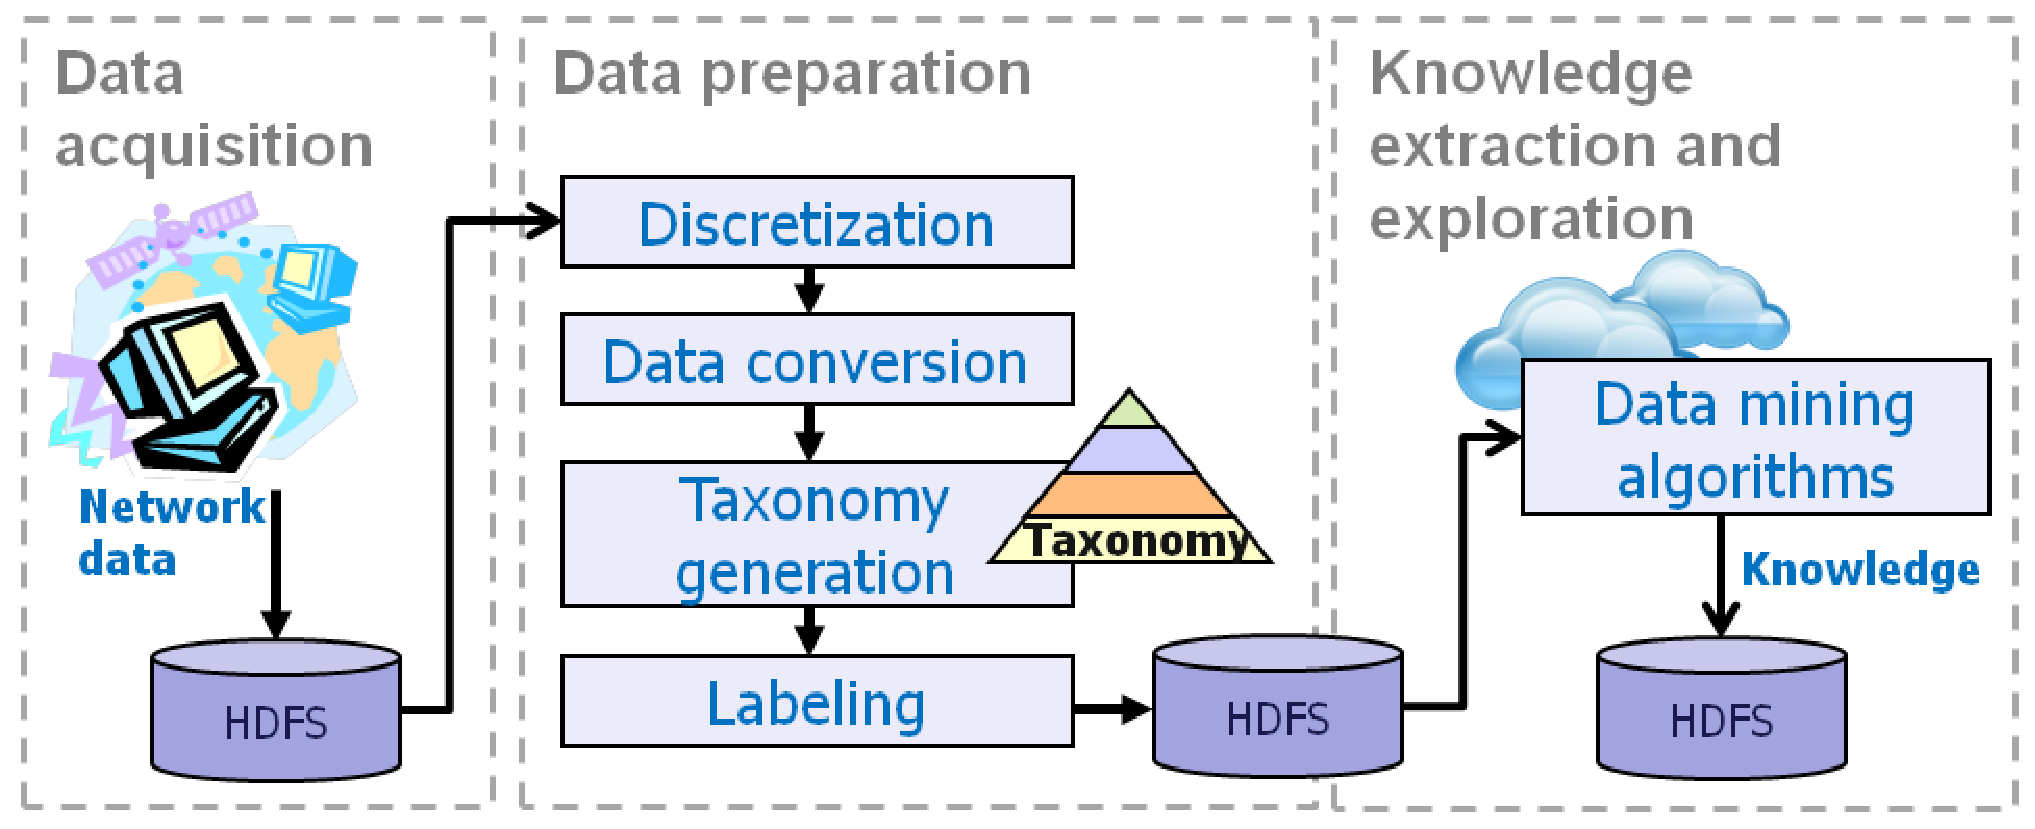
\includegraphics[width=0.49\textwidth]{Framework.eps}
\caption{Architecture of \Nemico}
\label{fig:arch}
\end{figure}



%****************************************************
\subsection{Data acquisition}
\label{Netacq}
%****************************************************

\Nemico\ acquires massive amounts of network traffic measurements through passive traffic sniffing.
A passive probe located on the Internet access link of an edge network is exploited to acquire incoming and outgoing packets flowing on the link.
Traffic monitoring is performed by Tstat~\cite{Tstat}, a tool that allows users to collect network and transport layer measurements. 
%Tstat rebuilds TCP connections by matching sequence numbers on data segments with the corresponding acknowledgement (ACK) numbers.
The acquired datasets consist of a set of records, each one corresponding to a different TCP flow.
To ensure measurement reliability, only the TCP flows that last more than ten packets (i.e., the long-lived flows) are considered.

\Nemico\ stores the collected network traffic data in an HDFS distributed file
system.  It can successfully acquire and handle all the network measurements provided by Tstat (i.e., the Round-Trip-Time (RTT) observed on a TCP flow, the class of application layer service (e.g., HTTP,VIDEO) assigned by Tstat). 

%Among others, the supported measurements comprise (i) the Round-Trip-Time (RTT) observed on a TCP flow, which indicates the minimum time lag between the observation of a TCP segment and the observation of the corresponding ACK, (ii) the TCP port of the server, (iii) the number of packets, and (iv) the class of application layer service (e.g., HTTP,VIDEO) assigned by Tstat. Note that Tstat measurements comprise both continuous values (e.g., the RTT) and discrete values (e.g., the class of service).  

%****************************************************
\subsection{Data preparation}
\label{dataprep}
%****************************************************

To suit the raw data to the subsequent data mining step some established data preprocessing steps are applied to the raw network traffic measurements. 
A brief description of the main data preparation steps is given below.

\textbf{Discretization}. Discretization concerns the transformation of continuous values into discrete ones. Since some data mining algorithms are unable to cope with continuously valued data, 
measurement values are discretized prior to running the algorithms. 
%In some cases (e.g., the association rule mining algorithms) discretization is not mandatory but strongly recommended because considering continuously valued attributes could bias the mining result (e.g., the association rules extracted from continuously valued attributes are unlikely to occur frequently in the source data). 
The discretization step can be performed either automatically by using established techniques~\cite{libroKumar} or semi-automatically by partitioning continuous value ranges into appropriate bins based on the prior knowledge about the measurement domains. 
%Due to the nature of the analyzed network data, manual data discretization is commonly preferable.  

\textbf{Data conversion}. Since most algorithms are designed to handle only a subset of specific data formats, data conversion entails the transformation of the raw data into the expected data format. For example, most association rule mining algorithms are designed to cope with transactional data~\cite{libroKumar}. Hence, to apply association rule mining algorithms the acquired data have to be tailored to the transactional data format. 

\textbf{Taxonomy generation}. The data mining process can be driven by semantics-based models (e.g., taxonomies or ontologies). These models are used to enrich the source data with multiple-level or multi-faceted information.  
For example, a taxonomy consists of set of is-a hierarchies built over the data attributes, which can be exploited to aggregate specific data values (e.g., the TCP ports) into meaningful higher-level categories.
Since many data mining algorithms (e.g.,~\cite{ISPA14}) allow pushing taxonomy-based information into the extraction process, \Nemico\ supports both
the automatic taxonomy inference over a subset of specific network data attributes (e.g., port number, packet number) 
and the semi-automatic taxonomy construction. 
%The mining process for extracting more abstract and interesting correlations among data (e.g., generalized association rules) is driven by taxonomies. 
%A taxonomy is a hierarchy of aggregations over values of one attribute (e.g., TCP port) and it is usually represented as a tree. 
%\Nemico\ allows either to automatically infer interesting taxonomies directly from the data. 
%To this aim different algorithms have been devised and implemented to automatically extract taxonomies for the considered attributes (i.e., port number, packet number) since some attributes (e.g., port number) are actually hierarchical attributes while others are numerical ones.
%In \Nemico\ taxonomies could also be provided directly by the user.

\textbf{Labeling}. Supervised data mining techniques (e.g., classification) require the labeling of one data attribute 
as class label. Hence, if the data mining process comprises supervised analyses domain-experts have to specify the class attribute. 


The current implementation of \Nemico\ includes a first implementation of all the described activities as map jobs.



\comment{The current implementation of \Nemico\ includes the implementation of both data discretization and conversion which are performed by a single map only job. Each record is processed by the map
function and, if the number of packets is above the threshold (e.g., 10 packets), the corresponding discretized version is generated as output of the mapping step.
This task entails an inherently parallel elaboration, considering that can be applied independently to each record.}



%****************************************************
\subsection{Knowledge extraction and exploration}
\label{KnowExt}
%****************************************************
Knowledge extraction entails the application of data mining algorithms to find implicit, previously unknown, and potentially useful information from large volumes of network data. 
\Nemico\ comprises novel data mining algorithms that contribute to a paradigm-shift in distributed data mining. The analytics algorithms entail (i) discovering underlying correlations among traffic data 
(e.g., multiple-level associations among data equipped with taxonomies), (ii) grouping traffic flows with similar properties (e.g., clustering), and (iii) extracting models useful for prediction (e.g., classification, regression).  
The algorithms are designed to address the following issues.

\textit{Sparse data distribution.} Since Big data collections have large cardinality and/or a high number of dimensions, they are usually characterized by an
inherent sparseness. Aimed at addressing this issue, we propose incremental algorithms that are able to cope with result refinement over different incremental runs
and that scale by adapting to new data without the need for re-analyzing the entire dataset.

\textit{Algorithm optimization}. Most data mining algorithms are poorly optimized for cloud computing environments. 
Conversely, our algorithms have specifically been designed to scale %improve the scalability of the existing techniques and their performance 
in massively parallel computing environments.

\textit{Horizontal scalability.} To apply the data mining techniques to petabyte-scale network traffic datasets, \Nemico\ integrates advanced analytics algorithms (e.g., association rule mining) with horizontally scalable approaches, 
such as those based on Map Reduce and shared columnar storage backends.

The current implementation of \Nemico\ comprises Hadoop-based data mining algorithms focused on the extraction of interesting and multiple-level correlations among network data (i.e., association rules~\cite{ISPA13} and 
misleading multiple-level patterns~\cite{ISPA14}). To make the results manageable for manual inspection the extracted patterns can be ranked according to established quality measures~\cite{libroKumar} 
to select top-k interesting ones or categorized into semantically related groups (e.g., all patterns related to a specific class of service).
Both input data and generated knowledge are stored in an HDFS file system. 

%**********************************************************
%\subsection{Knowledge categorization and selection}
%\label{KnowCatSel}
%**********************************************************
%Explorative data mining approaches, such as association rule mining and clustering algorithms, may identify interesting knowledge, which may be both huge in size and complex in structure. To ease exploitation of the mined knowledge, different
%interestingness measures (e.g., chi square, support expectation, collective strength) to reduce and evaluate the amount of extracted knowledge  are  needed. For a detailed review on measures for interesting rules and quality indexes for clustering see \cite{Hilderman2001} and  \cite{KumarBook} respectively. The current implementation of \Nemico\ includes COSA METTIAMO??

%Furthermore, only for the discovery of correlations when coping with relatively
%large or complex transactional network datasets the number of mined rules could be
%so large that a manual inspection becomes unfeasible. To overcome this issue, \Nemico\ propose a classification of the rules into
%groups according to their semantics in the network domain. 

%**********************************************************
\section{Experiments and conclusions}
\label{conc}
%**********************************************************

The current implementation of \Nemico\ was developed in Java using the new Hadoop Java APIs. It was validated on real network traffic datasets with size 192.56 GB. The experiments were performed on a cluster of 5 nodes running the Cloudera's
Distribution of Apache Hadoop (CDH4.5). More details of both cluster node and data can be found in \cite{ISPA14}. 
For both data mining algorithms in \Nemico , we evaluated the speedup achieved increasing the number of Hadoop cluster nodes and the achieved results show that our approaches scale roughly linearly with the number of nodes and the speedup approximately
corresponds to the number of cluster nodes. As future work we are planning to introduce visualization tools and new data mining algorithms to support
a larger variety of traffic data analyses. 

% An example of a floating figure using the graphicx package.
% Note that \label must occur AFTER (or within) \caption.
% For figures, \caption should occur after the \includegraphics.
% Note that IEEEtran v1.7 and later has special internal code that
% is designed to preserve the operation of \label within \caption
% even when the captionsoff option is in effect. However, because
% of issues like this, it may be the safest practice to put all your
% \label just after \caption rather than within \caption{}.
%
% Reminder: the "draftcls" or "draftclsnofoot", not "draft", class
% option should be used if it is desired that the figures are to be
% displayed while in draft mode.
%
%\begin{figure}[!t]
%\centering
%\includegraphics[width=2.5in]{myfigure}
% where an .eps filename suffix will be assumed under latex, 
% and a .pdf suffix will be assumed for pdflatex; or what has been declared
% via \DeclareGraphicsExtensions.
%\caption{Simulation Results}
%\label{fig_sim}
%\end{figure}

% Note that IEEE typically puts floats only at the top, even when this
% results in a large percentage of a column being occupied by floats.


% An example of a double column floating figure using two subfigures.
% (The subfig.sty package must be loaded for this to work.)
% The subfigure \label commands are set within each subfloat command, the
% \label for the overall figure must come after \caption.
% \hfil must be used as a separator to get equal spacing.
% The subfigure.sty package works much the same way, except \subfigure is
% used instead of \subfloat.
%
%\begin{figure*}[!t]
%\centerline{\subfloat[Case I]\includegraphics[width=2.5in]{subfigcase1}%
%\label{fig_first_case}}
%\hfil
%\subfloat[Case II]{\includegraphics[width=2.5in]{subfigcase2}%
%\label{fig_second_case}}}
%\caption{Simulation results}
%\label{fig_sim}
%\end{figure*}
%
% Note that often IEEE papers with subfigures do not employ subfigure
% captions (using the optional argument to \subfloat), but instead will
% reference/describe all of them (a), (b), etc., within the main caption.


% An example of a floating table. Note that, for IEEE style tables, the 
% \caption command should come BEFORE the table. Table text will default to
% \footnotesize as IEEE normally uses this smaller font for tables.
% The \label must come after \caption as always.
%
%\begin{table}[!t]
%% increase table row spacing, adjust to taste
%\renewcommand{\arraystretch}{1.3}
% if using array.sty, it might be a good idea to tweak the value of
% \extrarowheight as needed to properly center the text within the cells
%\caption{An Example of a Table}
%\label{table_example}
%\centering
%% Some packages, such as MDW tools, offer better commands for making tables
%% than the plain LaTeX2e tabular which is used here.
%\begin{tabular}{|c||c|}
%\hline
%One & Two\\
%\hline
%Three & Four\\
%\hline
%\end{tabular}
%\end{table}


% Note that IEEE does not put floats in the very first column - or typically
% anywhere on the first page for that matter. Also, in-text middle ("here")
% positioning is not used. Most IEEE journals/conferences use top floats
% exclusively. Note that, LaTeX2e, unlike IEEE journals/conferences, places
% footnotes above bottom floats. This can be corrected via the \fnbelowfloat
% command of the stfloats package.


% conference papers do not normally have an appendix


% use section* for acknowledgement
%\section*{Acknowledgment}

% trigger a \newpage just before the given reference
% number - used to balance the columns on the last page
% adjust value as needed - may need to be readjusted if
% the document is modified later
%\IEEEtriggeratref{8}
% The "triggered" command can be changed if desired:
%\IEEEtriggercmd{\enlargethispage{-5in}}

% references section

% can use a bibliography generated by BibTeX as a .bbl file
% BibTeX documentation can be easily obtained at:
% http://www.ctan.org/tex-archive/biblio/bibtex/contrib/doc/
% The IEEEtran BibTeX style support page is at:
% http://www.michaelshell.org/tex/ieeetran/bibtex/
%\bibliographystyle{IEEEtran}
% argument is your BibTeX string definitions and bibliography database(s)
%\bibliography{IEEEabrv,../bib/paper}
%
% <OR> manually copy in the resultant .bbl file
% set second argument of \begin to the number of references
% (used to reserve space for the reference number labels box)


\bibliographystyle{IEEEtran} 
\bibliography{biblio}

% that's all folks
\end{document}


